%
% Documento: Fundamentação Teórica
%

\chapter{Fundamentação Teórica}
\label{chap:fundamentacaoTeorica}

Para se obter grandes resultados na otimização de \textit{front-end} de \textit{websites} é essencial ter conhecimento de como o protocolo HTTP evoluiu e como ele funciona assim é possível encontrar seus pontos fracos e trabalhar em maneiras para minimizá-los. Além disso é necessário compreender o que são as chamadas assíncronas de JavaScript e XML, conhecidas como AJAX, e porque elas são tão utilizadas em \textit{websites} e aplicações para a chamada Web 2.0.

\section{O Protocolo HTTP}
\label{sec:http}

\section{História}
\label{sec:http_historia}

Em 1989 Tim Berners-Lee propôs uma rede de computadores global para ajudar a comunidade científica a compartilhar o conhecimento gerado em diferentes partes do mundo, acelerando assim o desenvolvimento tecnológico. Ao final de 1990 o cientista do CERN já tinha desenvolvido em um computador de seu laboratório o primeiro navegador \textit{web} (chamado de WorldWideWeb), uma linguagem de marcação de hipertextos (o HTML) e um protocolo para a transferência de hipertextos (o HTTP).

O HTTP recebeu sua primeira documentação oficial em 1991, quando passou a ser chamado de HTTP/0.9. Como esclarece \cite{HighPerformanceBrowserNetworking}, todas as versões anteriores passaram a ser consideradas iterações com o objetivo de se chegar a versão HTTP/0.9, então todas elas acabaram recebendo o rótulo de HTTP/0.9.

Essa primeira versão do protocolo era extremamente simples. A ideia é explicada por \cite{HighPerformanceBrowserNetworking} da seguinte maneira:

\begin{itemize}
	\item Uma conexão TCP é aberta
	\item A requisição do cliente é uma cadeia simples de caracteres ASCII
	\item A resposta do servidor é uma torrente de caracteres ASCII
	\item A resposta do servidor é um HTML
	\item A conexão é fechada após o transferência do documento 
\end{itemize}

Com o passar dos anos a \textit{World Wide Web} de Tim Berners-Lee cresceu rapidamente e isso fez com que o uso do HTTP aumentasse muito em pouco tempo. Viu-se a necessidade de um protocolo mais robusto e estruturado, mas que mantivesse a simplicidade do HTTP/0.9, pois esse era o segredo por trás de seu sucesso. Então o IETF  passou a coordenar a criação de especificações para o HTTP e criou o HTTP-WG que tinha a função definir as especificações das versões seguintes do protocolo. Então, em 1996 foi definido o HTTP/1.0 \cite{RFC1945}, em 1999 o HTTP/1.1 \cite{RFC2616} e em 2015 foi aprovada a especificação para o HTTP2 \cite{HTTP2Spec}.

\section{Visão Geral}
\label{sec:http_visão_geral}

Como dito por \cite{Tanenbaum}, o HTTP é um simples protocolo de requisições e respostas que normalmente funciona em cima do protocolo TCP. As requisições e respostas são compostas por um cabeçalho e um conteúdo, e são enviadas do cliente para o servidor. O HTTP é um protocolo independente de estado, ou seja, cada tupla requisição-resposta pode ser tratada de maneira independente, sem que as anteriores e futuras interfiram nela. O modelo, ilustrado na \autoref{fig:httpoverview}, é bem simples e direto, fácil de ser replicado.

\begin{figure}[!htb]
    \centering
    \caption{Visão Geral do Protocolo HTTP}
    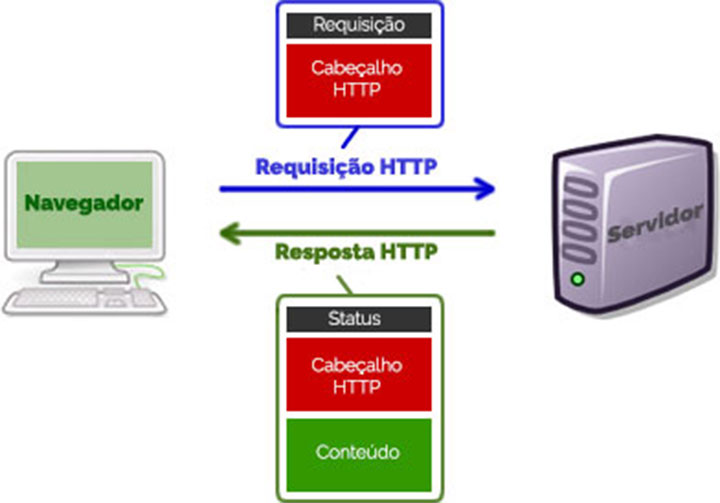
\includegraphics[width=0.6\textwidth]{./04-figuras/fund-teorica/http_overview}
    \fonte{Adaptado de  \citeonline{ImagemHTTPOverview}}
    \label{fig:httpoverview}
\end{figure}

O HTTP foi desenvolvido para funcionar na camada de Aplicação do protocolo TCP, conectando as ações do usuário a camada de Apresentação. Contudo, de acordo com \cite{Tanenbaum}, ele se transformou em um protocolo da camada de Transporte, criando uma maneira de processos se comunicarem através de diferentes redes. Hoje em dia não são apenas os navegadores \textit{web} que utilizam o protocolo HTTP para se comunicar com servidores, tocadores de mídias, anti-vírus, programas de fotos, dentre outros tipos de aplicações utilizam o HTTP para recolher informações de servidores de maneira simples e rápida.

Os cabeçalhos HTTP definem características desejadas ou esperadas pelas aplicações e servidores, como tipo de codificação de caracteres ou tipo de compressão dos dados. Existem várias etiquetas padrões que podem ser utilizadas nos cabeçalhos e os desenvolvedores podem ainda criar etiquetas próprias para serem utilizadas dentro das aplicações - por definição, caso um cliente ou servidor receba uma etiqueta que não reconhece ele simplesmente a ignora. No \autoref{qua:cabecalhoshttp} são apresentadas algumas das etiquetas mais utilizadas, mas existem muitas outras que não foram citadas e que podem variar com a versão do protocolo.

\begin{quadro}[!htb]
	\centering
	\caption{Etiquetas para cabeçalhos HTTP.\label{qua:cabecalhoshttp}}
	\begin{tabular}{| c | c | c |}
		\hline
		\textbf{Etiqueta} & \textbf{Tipo} & \textbf{Conteúdo}                                       \\
		\hline
		\textit{Accept}             & Requisição    & Tipo de páginas que o cliente suporta                   \\
		\hline
		\textit{Accept-Encoding}    & Requisição    & Tipo de codificação que o cliente suporta               \\
		\hline
		\textit{If-Modified-Since}  & Requisição    & Data e hora para checar atualidade do conteúdo          \\
		\hline
		\textit{Authorization}      & Requisição    & Uma lista de credenciais do cliente                      \\
		\hline
		\textit{Cookie}             & Requisição    & Cookie definido previamente enviado para o servidor     \\
		\hline
		\textit{Content-Encoding}   & Resposta      & Como o conteúdo foi codificado (e.g. \textit{gzip})               \\
		\hline
		\textit{Content-Length}     & Resposta      & Tamanho da página em \textit{bytes}                              \\
		\hline
		\textit{Content-Type}       & Resposta      & Tipo de \textit{MIME} da página                                  \\
		\hline
		\textit{Last-Modified}      & Resposta      & Data e hora que a página foi modificada pela última vez \\
		\hline
		\textit{Expires}            & Resposta      & Data e hora quando a página deixa de ser válida         \\
		\hline
		\textit{Cache-Control}      & Ambas          & Diretiva de como tratar \textit{cache}                           \\
		\hline
		\textit{ETag}               & Ambas          & Etiqueta para o conteúdo da página                      \\
		\hline
		\textit{Upgrade}            & Ambas          & O novo protocolo para o qual o cliente deseja alterar        \\	
		\hline
	\end{tabular}
	\fonte{Adaptado de \citeonline{Tanenbaum}}
\end{quadro}

O conteúdo de uma resposta HTTP pode assumir diferentes formatos (HTML, CSS, JavaScript, etc), a definição desse formato é feita com a etiqueta \textit{Content-Type} enviada no cabeçalho de resposta. O conteúdo é a maior parte de uma resposta HTTP e os desenvolvedores devem se esforçar para reduzi-lo ao máximo, garantindo que a comunicação de dados seja rápida e eficiente.

Por rodar em cima do protocolo TCP o HTTP precisa que uma conexão TCP seja aberta para poder realizar a troca de dados entre o cliente e o servidor. Como essa conexão é gerenciada vai depender da versão do protocolo. Após a abertura da conexão a requisição pode ser enviada. Na primeira linha da requisição são definidas a versão do protocolo e a operação que será realizada. Apesar de ter sido criado apenas para recuperar páginas \textit{web} de um servidor, o HTTP foi intencionalmente desenvolvido de forma genérica, possibilitando a extensibilidade do seu uso. Sendo assim o protocolo suporta diferentes operações, chamadas de métodos, além da tradicional requisição de páginas \textit{web}. A lista completa de métodos com suas descrições pode ser vista no \autoref{qua:metodoshttp}, vale ressaltar que esses métodos são \textit{case sensitive}, ou seja, o método \textit{get}, por exemplo, não existe.

\begin{quadro}[H]
	\centering
	\caption{Métodos HTTP.\label{qua:metodoshttp}}
	\begin{tabular}{| c | c |}
		\hline
		\textbf{Método} & \textbf{Descrição}							 \\
		\hline
		GET             & Ler página \textit{web}					             \\
		\hline
		HEAD            & Ler cabeçalho de página \textit{web}					 \\
		\hline
		POST            & Anexar à página \textit{web}					         \\
		\hline
		PUT             & Armazenar página \textit{web}                            \\
		\hline
		DELETE          & Remover página \textit{web }                             \\
		\hline
		TRACE           & Imprimir requisição de entrada                  \\
		\hline
		CONNECT         & Conectar através de um \textit{proxy}                    \\
		\hline
		OPTIONS         & Listar opções para uma página \textit{web}               \\
		\hline
	\end{tabular}
	\fonte{Adaptado de \citeonline{Tanenbaum}}
\end{quadro}

Dos citados no \autoref{qua:metodoshttp} os métodos GET e POST são os mais utilizados pelos navegadores \textit{web} e serão os mais utilizados neste trabalho. O método GET é utilizado para recuperar informações do servidor e o método POST para enviar informações para o servidor.

Sempre que uma requisição é enviada ela recebe uma resposta, mesmo que a requisição falhe. Na primeira linha do cabeçalho de resposta se encontra o código do estado da resposta em formato numérico de três dígitos. O primeiro digito deste código define a qual sub-grupo ele pertence. O \autoref{qua:estadoshttp} mostra os sub-grupos existentes e o significado de cada um deles. Cada um destes sub-grupos possui vários códigos  com diferentes significados e com a evolução do protocolo mais códigos foram sendo inseridos para lidar com necessidades especificas.

\begin{quadro}[!htb]
	\centering
	\caption{Códigos de estado HTTP.\label{qua:estadoshttp}}
	\fonte{Adaptado de \citeonline{Tanenbaum}}
\end{quadro}
\begin{table}[]
\centering
\caption{My caption}
\label{my-label}
\begin{tabular}{|l|l|l|}
\hline
\textbf{Código} & \textbf{Significado} & \textbf{Exemplo}                                                                                   \\ \hline
1xx             & Informação           & \begin{tabular}[c]{@{}l@{}}100 = servidor concorda em lidar\\ com requisição do cliente \end{tabular} \\ \hline
2xx             & Sucesso              & \begin{tabular}[c]{@{}l@{}}200 = sucessona requisição\\ 204 = nenhum conteúdopresente\end{tabular} \\ \hline
3xx             & Redirecionamento     & \begin{tabular}[c]{@{}l@{}}301 = página foi movida\\ 304 = \textit{cache} ainda é válida\end{tabular}       \\ \hline
4xx             & Erro do cliente      & \begin{tabular}[c]{@{}l@{}}403 = página proibida\\ 404 = página não encontrada\end{tabular}        \\ \hline
\end{tabular}
\end{table}
	

A \textit{cache} é uma característica importante do HTTP. O protocolo foi construído com suporte integrado para lidar com este requisito de desempenho. Os clientes e os servidores conseguem gerenciar \textit{caches} com a ajuda dos cabeçalhos de requisição e resposta, mas o tamanho da \textit{cache} é definido pelo navegador. O problema destas memórias locais é saber o momento de utilizar os dados armazenados nelas ou de pedir novos dados ao servidor. Para isso existem variadas técnicas, como as propostas por \cite{HighPerformance}, que devem ser analisadas e utilizadas de acordo com a situação.

As versões do protocolo HTTP foram aprimorando falhas identificadas quando ele passou a ser utilizado em larga escala. Mas apesar das mudanças a essência do protocolo continua a mesma: um simples protocolo de requisição e resposta. Nas próximas seções serão apresentadas comparações entre as versões do HTTP, com ênfase nas mudanças que ajudaram a melhorar a performance dos \textit{websites} e aplicações \textit{web}.

\section{HTTP/1.0 VS HTTP/1.1}
\label{sec:http_10_vs_http_11}

Com a popularização da Internet na década de 1990 o uso do HTTP estava cresceu rapidamente. Com isso o IETF teve que se apressar para criar um documento de consulta para desenvolvedores que queriam utilizar o protocolo em suas aplicações. Sendo assim, apesar de todo o debate por trás da \cite{RFC1945}, aprovada em 1996, o documento apenas explicou os usos comuns do HTTP/1.0, mas não chegou a definir padrões de como utiliza-lo, como explica \cite{KeyDifferencesHTTP}. Por isso logo após a sua aprovação o HTTP-WG já começou a trabalhar na \cite{RFC2616}, para poder corrigir os erros existentes no HTTP/1.0 com a criação de uma nova versão, o HTTP/1.1.

Várias funcionalidades importantes foram adicionadas no HTTP/1.1, e existiu uma preocupação muito grande com a compatibilidade entre as versões do protocolo, afinal de contas o HTTP/1.0 já era amplamente utilizado e não podia se esperar que todos os \textit{websites} e aplicações se adaptassem de uma hora para outra. Esse fato também levou o HTTP-WG a criar um protocolo que suportasse mudanças futuras (lembrando que no HTTP todas as etiquetas que um cliente ou servidor não reconhecem são simplesmente ignoradas). Pensando na extensibilidade do protocolo as primeiras mudanças no protocolo HTTP/1.1 que valem ser citadas foram a criação de duas novas etiquetas para cabeçalhos, \textit{Upgrade} - uma maneira do cliente informar qual versão do protocolo ele suporta - e \textit{Via} - que define uma lista dos protocolos suportados pelos clientes ao longo do caminho de uma transmissão.

Como dito anteriormente o protocolo HTTP foi construído com suporte integrado para \textit{cache}. Mas o mecanismo de \textit{cache} do HTTP/1.0 era muito simples e não permitia que o cliente ou o servidor definisse instruções diretas de como a memória deveria ser utilizada. O HTTP/1.1 tentou corrigir esse problema com a criação de novas etiquetas para cabeçalhos. A primeira delas é a \textit{ETag}, que define uma cadeia de caracteres única para um arquivo. Além do próprio conteúdo, essa cadeia utiliza a data e a hora da última modificação no arquivo, logo pode ser utilizada para verificar se dois arquivos são idênticos. O HTTP/1.1 também definiu novas etiquetas condicionais para complementar a já existente \textit{If-Modified-Since}. As etiquetas \textit{If-None-Match}, \textit{If-Match} e \textit{If-Unmodified-Since}, passaram a poder ser usada para verificar se arquivos em \textit{cache} estão atualizados ou não. Uma das mudanças mais significativas no mecanismo de \textit{cache}, foi a etiqueta \textit{Cache-Control} que permiti definir novas diretrizes para o uso da \textit{cache}, como tempo de expiração relativos e arquivos que não devem ser armazenados.

O HTTP/1.0 tinha muitos problemas em gerenciar a largura de banda, por exemplo não era possível enviar partes de arquivos, logo, mesmo se o cliente não precisasse de um arquivo inteiro, ele teria de recebe-lo. No HTTP/1.1 foram então criados a etiqueta \textit{Range}, o tipo \textit{MIME} \textit{multipat/byteranges} e o tipo de compressão \textit{Chuncked} para que cliente e servidores pudessem trocar mensagens com partes de arquivos. Para complementar esse novo mecanismo foi incluído um novo código de resposta, 100, que informava um cliente que o corpo de sua requisição deve ser enviado. Além de poder enviar partes de arquivos o HTTP/1.1 se preocupou em garantir a compressão dos dados durante todo o caminho da transmissão, então foi incluída a etiqueta \textit{Transfer-Encoding}, que complementa a \textit{Content-Encoding} indicando qual codificação foi utilizada na transmissão ponto a ponto.

O modelo original do protocolo HTTP utilizava uma conexão TCP para cada transmissão. Esse processo era extremamente danoso para o desempenho de \textit{websites} e aplicações, pois se gastava muito tempo na criação e configuração de novas conexões e nos momentos iniciais da conexão (quando, por definição, ela é mais lenta). Para corrigir esse problema o HTTP/1.1 define conexões persistentes como seu padrão. Conexões persistentes permitem que clientes e servidores assumam que uma conexão TCP continuará aberta após a transmissão de dados, e que esta poderá ser utilizada para uma nova transmissão. Além disso foi definido que o HTTP/1.1 utilizaria \textit{pipeline}, isto quer dizer que clientes não precisam aguarda a resposta de uma requisição para mandarem uma nova requisição, como era o padrão do HTTP/1.0. Os ganhos com essas novas técnicas podem ser notados na \autoref{fig:httpconexaopersistente}.

\begin{figure}[!htb]
    \centering
    \caption{HTTP com (a) múltiplas conexões e requisições sequenciais. (b) Uma conexão persistente e requisições sequenciais. (c) Uma conexão persistente e requisições em pipeline}
    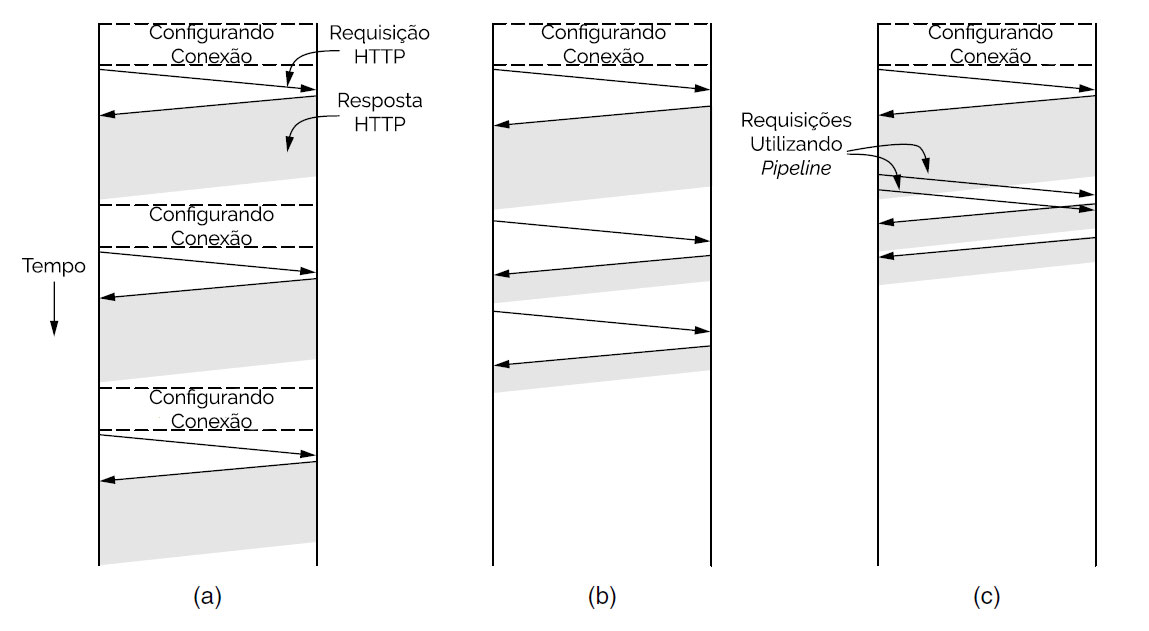
\includegraphics[width=1.0\textwidth]{./04-figuras/fund-teorica/httpconexaopersistente}
    \fonte{Adaptado de  \citeonline{Tanenbaum}}
    \label{fig:httpconexaopersistente}
\end{figure}

Uma funcionalidade desejada no HTTP/1.1 era a de poder fazer requisições para servidores outros além do da página principal sendo acessada. Isso possibilita que desenvolvedores hospedem arquivos CSS e JavaScript em um servidor e imagens em outro por exemplo. Isso se tornou possível com a adição da etiqueta \textit{Host}, onde o cliente pode definir que é o caminho do servidor que será utilizado na requisição. Caso a etiqueta \textit{Host} não esteja definida no cabeçalho é assumido que o caminho do servidor é o caminho da página principal.

Como conclui \cite{KeyDifferencesHTTP}: os protocolos HTTP/1.0 e HTTP/1.1 diferem em diversas maneiras. Enquanto muitas dessas mudanças têm o objetivo de melhorar o HTTP, a descrição do protocolo mais do que triplicou de tamanho, e muitas dessas funcionalidades foram introduzidas sem testes em ambientes reais. Esse aumento de complexidade causou muito trabalho para os desenvolvedores de clientes e servidores \textit{web}. 

No \autoref{qua:http11novo} encontra-se um resumo das mudanças introduzidos no protocolo HTTP/1.1. Observa-se que nem todas as mudanças mostradas no \autoref{qua:http11novo} foram detalhadas anteriormente, mas servem para ilustrar que existem ainda outras diferenças entre as versões 1.0 e 1.1 do protocolo que para os fins deste trabalho elas não são relevantes.

\begin{quadro}[H]
	\caption{Mudanças introduzidas no HTTP/1.1}
	\centering
	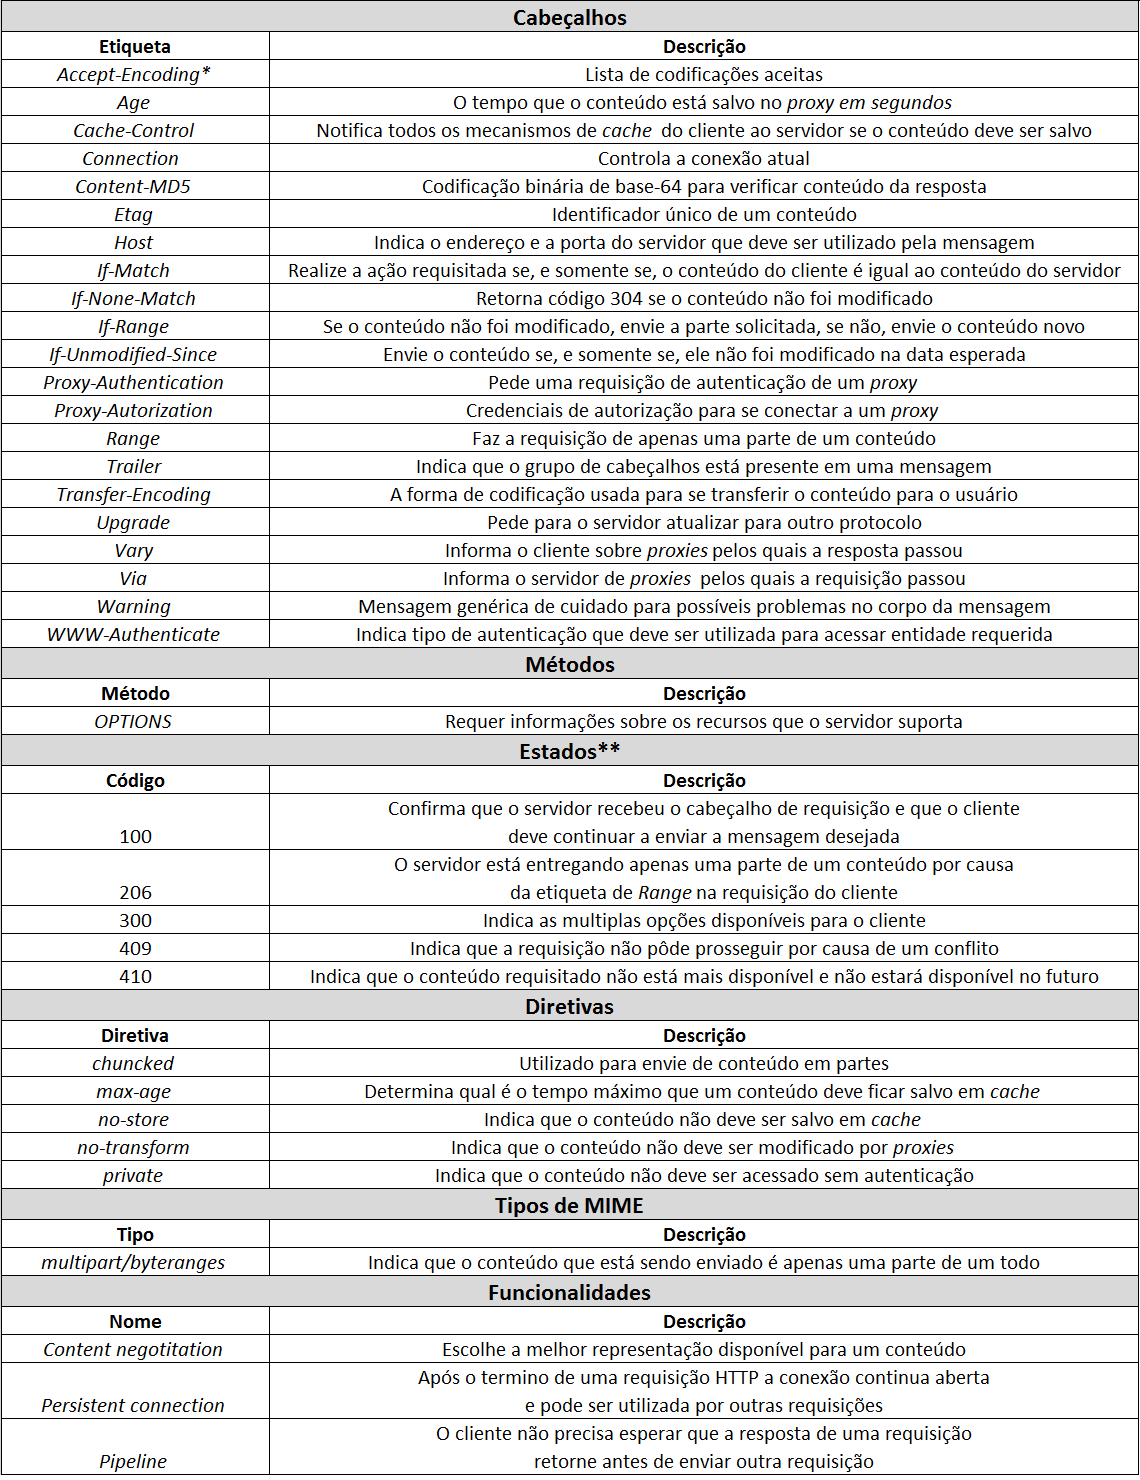
\includegraphics[width=1.0\textwidth]{./04-figuras/fund-teorica/http11novo}
	\label{qua:http11novo}
\end{quadro}


\section{HTTP/1.1 VS HTTP/2}
\label{sec:http_11_vs_http_2}

Com o lançamento do HTTP/1.1 apenas 3 anos depois do HTTP/1.0 o protocolo conseguiu se firmar e provou que seria o protocolo dominante da Internet. O HTTP/1.1 era robusto e flexível, permitindo que fosse utilizado em aplicações diversas de maneira eficiente. Com o passar dos anos o IETF acrescentou algumas extensões ao protocolo para corrigir erros pontuais, mas o HTTP suportava as necessidades da rede mundial de computadores.

No inicio do século XXI os \textit{websites} começaram a mudar. Eles passaram a se tornar mais complexos e consequentemente maiores, muitas fontes e folhas de estilo eram utilizadas e cada página passou a possuir vários arquivos de JavaScript. Além disso eles deixaram de ser estáticos e passaram a responder dinamicamente às ações dos usuários. Hoje em dia muitas requisições HTTP são necessárias para se montar uma página \textit{web} e essas requisições podem ser longas e demoradas. Finalmente o HTTP/1.1 passou a ser visto como um gargalo de desempenho para \textit{websites}, então em 2007 o IETF formou o grupo HTTPbis (onde o "\textit{bis}" quer dizer "de novo" em latim). Mas o grupo só começou as discussões sobre a nova verão do protocolo em 2012, terminando de redigir as especificações em 2014. Após revisões a especificação oficial da nova versão do HTTP vou aprovada no inicio do ano de 2015 e deve começar a ser utilizada em 2016. A nova versão do HTTP passou a se chamar  HTTP/2, sem os decimais, caso mudanças sejam necessárias será lançada uma nova versão completa do protocolo. 

O HTTP/2 veio para corrigir o problema de latência existente na versão anterior. Apesar do sistema de \textit{pipeline}, o HTTP/1.1 é muito sensível à latência, ou seja, apesar de conseguir entregar muitos dados existem problemas quanto ao tempo de viagem das requisições e respostas. Isso acontece porque o \textit{pipeline} do HTTP/1.1 é muito difícil de ser gerenciado e muitas vezes fecha conexões que deveriam ter ficado abertas. O problema é tão grande que \cite{HTTP2Explained} afirma que  mesmo nos dias de hoje muitos navegadores \textit{web} preferem desativar o \textit{pipeline}. Para corrigir este problema o HTTP/2 propõe mudanças na forma como as informações são enviadas. O mais importantes destas mudanças é que, assim como ocorreu das versões 1.0 para 1.1, elas não podem alterar nenhum paradigma já existente no protocolo. As aplicações que utilizam o HTTP/1.1 devem continuar funcionando no HTTP/2, os formatos de arquivos, as URL e as URI devem ser mantidos e o usuário final não deve ter de fazer nada para poder aproveitar das melhorias do novo protocolo. Com isso, para tentar criar um protocolo que funcionasse no mundo real tanto quanto no teórico, o HTTPbis decidiu se inspirar no protocolo SPDY, criado pela Google, por este já ter se provado um conceito funcionou.

A primeira mudança no HTTP/2 está na forma como ele escreve suas requisições e respostas. Em suas versões anteriores o protocolo optou por utilizar o formato ASCII para estruturar suas requisições e respostas, mas era difícil separar as partes dos cabeçalhos e tratar espaços em branco indesejados. Para resolver esse problema o HTTP/2 é um protocolo binário. Assim é mais simples quebrar requisições e respostas em quados, comparar quadros e comprimir as informações. Entre as desvantagens dessa representação binária estão o fato de que os cabeçalhos HTTP não serão mais compreensíveis sem a ajuda de ferramentas e que a depuração do protocolo dependerá de analisadores de pacotes.

Utilizando a presentação binária o HTTP/2 possibilita a multiplexação de \textit{streams} de dados. Como explica \cite{HTTP2Explained} Uma \textit{stream} é uma associação lógica criação por uma sequencia de quadros. No HTTP/2 uma conexão possui várias \textit{streams} e por isso vários componentes podem ser transferidos ao mesmo tempo. Para esse processo funcionar o protocolo multiplexa essas \textit{streams} no momento do envia e as separa novamente na chegada. A \autoref{fig:streamsmultiplexadas} ilustra a multiplexação de \textit{streams}.

\begin{figure}[!htb]
    \centering
    \caption{Multiplexação de \textit{strems} no HTTP/2 (a) duas \textit{streams} separadas (b) \textit{streams} multiplexadas}
    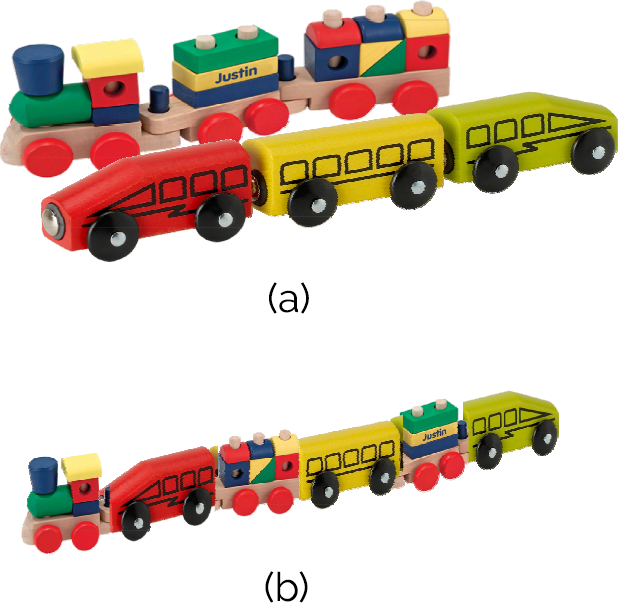
\includegraphics[width=1.0\textwidth]{./04-figuras/fund-teorica/multiplexed_streams}
    \fonte{Adaptado de  \citeonline{HTTP2Explained}}
    \label{fig:streamsmultiplexadas}
\end{figure}

Um problema no HTTP/1.1 era a garantia de que um componente A já teria sido baixado quando outro componente B que depende de A fosse executado. Apesar de o HTML garantir isso, essa limitação impedia que a paralelização de \textit{downloads} fosse maior. No HTTP/2 as foram adicionado os mecanismos de prioridade e dependência. Com eles é fácil indicar quais \textit{streams} devem ser baixado primeiro e quais são as dependências entre elas. Dessa forma os desenvolvedores podem paralelizar ao máximo seus componentes e o protocolo cuidará de evitar erros. 

A compressão de dados é um fator importante para o aumento de desempenho do HTTP. Com o passar dos anos as requisições e respostas aumentaram de tamanho, e as compressões criadas para o SPDY e o HTTPS não se provaram eficientes contra ataques de terceiros. Logo notou-se que este era um ponto crítico para a nova versão do protocolo, então o HTTPbis decidiu por criar o HPACK, que será o novo formato de compressão para cabeçalhos HTTP/2. Visando a robustez desse formato, foi criado uma nova especificação exclusivamente para o HPACK que detalha como ele funciona e como deve ser usado \cite{HPACKSpec}.

Assim como na versão anterior, o HTTP/2 possui mecanismos para lidar com a \textit{cache}. As etiquetas existentes no HTTP/1.1 continuam a existir, mas uma nova funcionalidade foi adicionada na nova versão, o \textit{Server Push}. A ideia por trás é garantir que o cliente consiga componentes da maneira mais rápida. Então se o cliente requisitar um componente X o servidor pode saber que é provável que ele vá requisitar o componente Y nos próximos instantes, sendo assim o servidor pode enviar o componente Y antes mesmo de receber o pedido por ele. Essa funcionalidade é algo que o cliente deverá especificar explicitamente, mas existe grande expectativa quando as melhorias que ela pode trazer. Além dessa melhoria no sistema de cache, o HTTP/2 inclui uma nova etiqueta para impedir o desperdício de banda de transmissão. Se o servidor começar a enviar um componente com um tamanho específico e perceber que aquele componente não é mais útil, ele pode cancelar o envio com a etiqueta \textit{RST STREAM}, evitando que a \textit{stream} de envio fique ocupada com dados desnecessários por muito tempo.

Caso um \textit{website} ou uma aplicação deseje transferir o cliente para outro servidor sem ser o requisitado, ou até mesmo para outra porta, ele poderá utilizar a etiqueta Alt-Svc. Com essa etiqueta o servidor informa ao cliente para onde ele deve ir, então o cliente deve tentar se conectar de maneira assíncrona no caminho sugerido pelo Alt-Svc e utilizar aquela conexão apenas se ela se provar confiável. Essa etiqueta foi criada com a intensão de informar clientes que os dados requisitados estão disponíveis também em um servidor seguro.

Como explicado anteriormente o HTTP/2 utiliza de \textit{streams} para enviar e receber dados. Esta técnica foi escolhida para aumentar a velocidade de envio do protocolo e a quantidade de dados que pode ser enviado de uma só vez. Cada uma dessas \textit{streams} possui sua própria janela de fluxo independente, o que garantirá que se uma \textit{stream} falhar as outras continuem funcionando. Para impedir o envia de dados e parar todas as \textit{streams} abertas, o protocolo inclui a etiqueta \textit{BLOCKED}, que informa que existem dados para serem enviados, mas algo está impedindo o processo de continuar.

O protocolo HTTP/2 trás grandes mudanças na estrutura dos dados que serão enviados e recebidos. A essência continua a mesma, um protocolo de requisições e respostas, mas a medida que o protocolo evolui novas formas de garantir o desempenhos dos \textit{websites} e das aplicações estão sendo acrescentadas ao HTTP. Neste trabalho foram detalhadas as mudanças que visaram melhoria de desempenho e que podem afetar a forma como a otimização de desempenho de \textit{websites} é feita. O documento completo com toda a especificação pode ser encontrado em \cite{HTTP2Spec}. O \autoref{qua:http2novo} mostra um resumo das mudanças detalhadas acima.

\begin{quadro}[H]
	\caption{Mudanças introduzidas no HTTP/2}
	\centering
	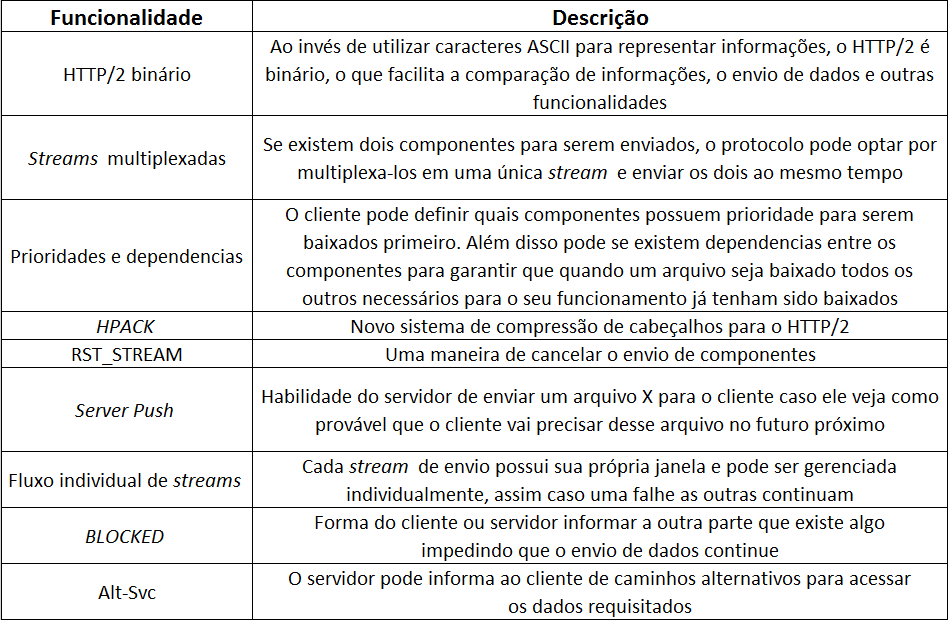
\includegraphics[width=1.0\textwidth]{./04-figuras/fund-teorica/http2novo}
	\label{qua:http2novo}
\end{quadro}

